%!TEX TS-program = xelatex
%!TEX encoding = UTF-8 Unicode
%!BIB TS-program = biber

\documentclass[12pt]{article}

\usepackage[colorlinks=true,linkcolor=blue,citecolor=blue,filecolor=blue,urlcolor=blue]{hyperref}

\usepackage{listings}

\usepackage{caption}
\usepackage{blindtext}
\captionsetup[table]{skip=5pt}

\usepackage[bottom]{footmisc}

\usepackage{expex}
\usepackage{setspace}
\usepackage{titlesec}
\usepackage{multicol}
\usepackage[noabbrev]{cleveref}

\titleformat*{\section}{\normalsize\bfseries}
\titleformat*{\subsection}{\normalsize\bfseries}
\titleformat*{\subsubsection}{\normalsize\bfseries}
% \titleformat*{\paragraph}{\large\bfseries}
% \titleformat*{\subparagraph}{\large\bfseries}

\usepackage{booktabs}

\usepackage[british]{babel}
\usepackage{csquotes}
\usepackage[backend=biber,natbib=true,style=apa]{biblatex}
\DeclareLanguageMapping{english}{british-apa}

\usepackage{mathspec}
\setromanfont{Minion Pro}

\usepackage{fullpage}

\newcommand{\burm}[1]{{\fontspec[Script=Myanmar]{Padauk}#1}}
\newcommand{\ipa}[1]{{\fontspec{Times New Roman}#1}}

\newcommand{\condc}{\textsc{citation }}
\newcommand{\condf}{\textsc{+focus }}
\newcommand{\condu}{\textsc{-focus }}

\addbibresource{burmese.bib}

\begin{document}

\noindent SPHL702 Report \vspace{0.25cm}

\noindent\Large An acoustic and electroglottographic study of Burmese nasals \vspace{0.5cm}

\normalsize\noindent Nay San

\normalsize

\onehalfspacing

\section{Method}
\label{sec:method}

All experimental stimuli, data, signal processing and statistical analysis code from this project are available on GitHub: \url{https://github.com/fauxneticien/BurmeseNasals}. References to this repository, 'BN', in the text will be displayed in monospaced type text such as \texttt{BN/experiment}.

\subsection{Participants} % (fold)
\label{sub:participants}

One 38-year old native female speaker of Burmese was recruited for this study. The speaker completed her entire school and university education in Mandalay, Burma and is fully literate in the language. She has been residing in Australia since 2006. The speaker reported having good vocal health.

\subsection{Stimuli} % (fold)
\label{sub:stimuli}

For each of the 4 nasal places of articulation (bilabial, alveolar, palatal, velar) in Burmese, there exists voiced and voiceless nasals \citep{okell1969reference}. Additionally, Burmese is a tonal language with 4 tone categories (creaky, low, high, checked). Thus, given a single vowel, e.g. \ipa{/a/}, there may be up to 32 potential lexical items of the form /Na/, e.g.: \ipa{/mà/} \emph{hard}, \ipa{/m̥à/} \emph{to order (buy)}, \ipa{/ŋ̥a̰/} \emph{to distribute equally}, etc. Using an online Burmese-English dictionary,\footnote{South-East Asian Languages Library: Burmese Lexicography, \url{http://sealang.net/burmese/dictionary.htm}} it was found that there were 25 lexical items of the form \ipa{/Na/}. A full list of items of this form, including the non-lexical items, is available in Appendix A: \Cref{tab:words}.

\subsection{Procedure} % (fold)
\label{sub:procedure}

\emph{Task conditions}. Previous studies on Burmese nasals have mainly elicited their target words in citation form \ipa{/Na/} tokens \citep{dantsuji1984study,dantsuji1986some,maddieson1984tono}, with the exception an oral-nasal airflow study by \citet{bhaskararao1991two} who used a carrier phrase \ipa{{[}ŋà \underline{\hspace{0.5cm}} kò jé nè tè{]}} \emph{I am writing \underline{\hspace{0.5cm}}}. \citet{tun1982some} suggests that eliciting citation form monosyllabic CV words from Burmese speakers may create an unnatural setting, as utterances in Burmese are accompanied by at least one (monosyllabic) particle (e.g. \mbox{\ipa{/é lá/}}, Cold$_{\textsc{adj}}$ \textsc{ Q}, \emph{ Are you cold?}). Accordingly, \citet{tun1982some} elicited vowels in \ipa{/hVdə/} nonce words for his study of tone. Following this line of reasoning, the items in the \condc condition for this present study were designed to be disyllabic nonce words of the form \ipa{/əNa/}. Following the design in \citet{bhaskararao1991two}, the \condf condition used the exact same carrier phrase. An additional \condu condition was added to examine the effect of prosody on the realisation of the nasal segments. In this condition, the participant was asked to place the nuclear stress on the verb \emph{write} instead of the object in the sentence, making it an answer to the question \emph{What are you doing with the word X? Ans: I am \textbf{writing} X.} \Cref{fig:conds} provides an overview of the three elicitation conditions. For each of the three conditions, there were 5 repetition blocks consisting of 32 trials. The trials were randomized and presented on a 2011 Apple Macbook Pro through an HTML web app, available at \texttt{BN/experiment}. A total of 480 \ipa{/Na/} tokens (32 trials $\times$ 5 blocks $\times$ 3 conditions) were elicited from the speaker.

\begin{figure}[t]
	\centering
	\begin{minipage}[t]{.20\linewidth}
		\textsc{citation}
		\exdisplay[everygla={},aboveexskip=1pt,belowexskip=1pt]
		\begingl
			\gla \burm{အနှာ}//
			\glb \ipa{ən̥à}//
			\glc  //
			\glft No meaning//
		\endgl
		\xe
	\end{minipage}
	\begin{minipage}[t]{.35\linewidth}
		\textsc{+focus}
		\exdisplay[everygla={},aboveexskip=1pt,belowexskip=1pt]
		\begingl
			\gla \burm{ငါ} {\burm{နှာကို}} {\burm{ရေးနေတယ်}}//
			\glb \ipa{ŋà} {\ipa{n̥à.kò}} {\ipa{jé.nè.tɛ̀}}//
			\glc I {nose.\textsc{obj}} write.\textsc{prog.real}//
			\glft \emph{I am writing 'nose'}//
		\endgl
		\xe
	\end{minipage}
	\begin{minipage}[t]{.40\linewidth}
		\textsc{-focus}
		\exdisplay[everygla={},aboveexskip=1pt,belowexskip=1pt]
		\begingl
			\gla \burm{ငါ} {\burm{နှာကို}} {\burm{\textbf{ရေး}နေတယ်}}//
			\glb \ipa{ŋà} {\ipa{n̥à.kò}} {\ipa{\textbf{jé}.nè.tɛ̀}}//
			\glc I {nose.\textsc{obj}} \textbf{write}.\textsc{prog.real}//
			\glft \emph{I am \textbf{writing} 'nose' (not reading it)}//
		\endgl
		\xe
	\end{minipage}
	\caption{The word \ipa{/n̥à/} \emph{nose} as it appeared within the three elicitation conditions used in the experiment.}
	\label{fig:conds}
\end{figure}

\emph{Experimental set up.} The recording session took place in a sound attenuated room at the Macquarie University Speech Physiology Lab. The electrodes of the electroglottograph (EGG) were self-placed by the participant under the guidance of the experimenter. The electrodes were connected to the input port of a Laryngograph microProcessor EGG-D200, produced by Laryngograph Ltd (London, UK). A generic PC microphone was attached the the 3.5 mm audio input of the EGG-D200 unit and placed approximately 5 cm below the participant's chin. The unit was connected via USB to an ASUS desktop PC running Windows 8. The Speech Studio software (Version 5.1.0, also produced by Laryngograph Ltd) was used to capture the input EGG and audio signals. As the Speech Studio software allowed for live monitoring of the signal, calibration took place by asking the participant to utter a sustained vowel \ipa{[a]} and adjusting the position of the electrodes until reasonably clean signals were acquired. After calibration, the participant read aloud the word list in \Cref{tab:words} to familiarise themselves with the items. The experiment began after 2 repetitions of the list. The data were saved and exported after each experimental block as a two channel WAV file sampled at 48 kHz per channel with 16-bit quantization.

\subsection{Analysis} % (fold)
\label{sub:analysis}

\subsubsection{Annotation environment} % (fold)
\label{sub:annotation}

The audio channels were extracted from the resulting WAV files and each of the 288 /Na/ tokens from blocks two, three and four (i.e. except the first and last blocks) were annotated in Praat \citep{boersma2002praat}. The segmentation process relied primarily on spectrographic and waveform information. The Praat spectrogram settings were kept the same throughout all the annotations: View range, 0-10 kHz; Window length, 0.005 s; Dynamic range, 40.0 dB. The waveform display used Praat's standard settings. Pitch, intensity and formant tracks displays were generally turned off and only used as secondary information when required. When these displays were activated, the settings were adjusted according to local information in order to find inflection points in the time course. All the Praat TextGrids are available at \texttt{BN/data/TextGrids}.

\subsubsection{Segmentation criteria} % (fold)
\label{sub:segmentation}

\vspace{1em}

\emph{Onset of nasal segments} (e.g. \Cref{fig:praat} at 4.8 ms, all tiers). In both voiced and voiceless nasals, the change in waveform complexity was used as a primary cue for the onset of the segments. In voiceless nasals with a voiceless component, an additional cue was the termination of F2 and higher frequencies. In the sentence conditions when these cues were less clear, pitch and intensity tracks were activated for supplementary information. It was observed that a local minimum in the pitch and intensity tracks consistently correlated with the first cycle in the waveform of a nasal segment.

\emph{Offset of voiceless components} (e.g. \Cref{fig:praat} at 16.9 ms, Voiceless tier). When voiceless nasals were produced with an evident voiceless component, the offset of voicelessness was annotated at the appearance of a voicing bar in the spectrogram and the onset of activity in the waveform. If there was no evident voiceless component (i.e. persistence of a voicing bar in throughout the voiceless nasal segment), then no annotations were placed on the Voiceless tier.

\newpage

\begin{figure}[ht!]
	\centering
	\includegraphics[scale=0.8]{figures/praat.eps}
	\caption{Annotated temporal boundaries of a token, \ipa{/n̥a̰/} \emph{how many}. The onset of the initial vowel \ipa{/ə/} was not annotated in the data and has been included in the figure for illustrative purposes.}
	\label{fig:praat}
\end{figure}

\emph{Offset of nasal segments} (e.g. \Cref{fig:praat} at 26.1 ms, Segment tier). The offset of nasal segments were primarily determined from their waveform and spectrographic properties. The increase in waveform complexity and termination of nasal anti-resonances were used to identify the nasal segment boundary. The palatal nasals proved considerably difficult to segment, especially in the sentence conditions, due to a high level of coarticulary effects during the nasal-vowel transition. In these cases, the mid-point between the last waveform cycle clearly identifiable as a nasal consonant and the first waveform cycle clearly identifiable as a vowel was taken to be the offset point.

\emph{Offset of post-consonantal vowel} (e.g. \Cref{fig:praat} at 44.1 ms, Segment and Item tiers). Although the vowels were not analysed in this study, the annotation process additionally placed an offset point for the vowels. In citation form, this was placed at the termination of F2 and higher frequencies. In the sentence conditions, the offset was placed at the beginning of the stop closure of the following word \ipa{/kò/}. When the object marker \ipa{/kò/} was not fully realised, as is common in rapid speech, the intensity track was used to find a local minimum corresponding to some form of residual stricture from the \ipa{/kò/} utterance.

\subsubsection{Acoustic measures} % (fold)
\label{sub:acoustic_measures}

The Praat TextGrid data were converted and stored in a SQLite database in order to conduct acoustic measures over the annotated intervals. For each nasal segment, a \texttt{matlab\_start} and \texttt{matlab\_end} time point was defined. For voiced nasals, this was equivalent to the start and end times of the segment. For voiceless nasals, \texttt{matlab\_end} was equivalent to the end time of the segment while \texttt{matlab\_start} was defined at the offset of voicelessness if an evident voiceless interval had been annotated in the data. That is, acoustic measures were only conducted on the voiced portions of voiceless nasals.

The first, second and third formants (F1, F2, F3) were obtained by using the FormantMeasurer software \citep{morisson2011formant}, which derives 6 candidate sets of F1, F2 and F3 tracks, and selects them according to a number of heuristics. The output consists of three time series tracks for each formant at 2 ms intervals. A step-by-step description of the algorithm is available in \citet{zhang2013reliability}. Pitch (F0) tracks of the acoustic data were obtained using a \textsc{Matlab} implementation of the Praat pitch tracker \citet{boersma1993accurate}. The data extraction script is available at \texttt{BN/analyses/matlab.m} and the resulting raw data in the SQLite database \texttt{BN/data/matlab.sqlite}.

\subsubsection{EGG measures} % (fold)
\label{sub:egg_measures}

The EGG data for each of the experimental blocks, containing 32 tokens each, were imported into \textsc{Matlab} and smoothed using the \texttt{smooth} function with a window span value of 20. This value was found to be the minimum window that allowed the peak detection algorithm\footnote{\texttt{peakdet} by Eli Billauer. Retrieved from \url{http://www.billauer.co.il/peakdet.html}} to function correctly without returning erroneous peaks. After the global smooth of the entire block signal, data points corresponding to the voiced portions of each nasal segment were extracted.

\begin{figure}[h]
	\centering
	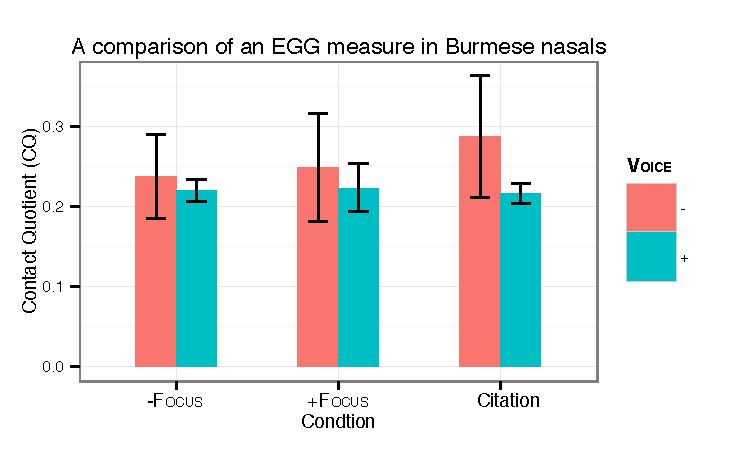
\includegraphics[width=6.5in]{figures/egg.eps}
	\caption{Calculation of peaks, troughs, and left and right points (10\% above the trough relative to amplitude difference between a trough and the prior peak). Cycles were defined to be a set of 5 time points starting from the first right point.}
	\label{fig:eggm}
\end{figure}

For each of the extracted signals, time points corresponding to all peaks and troughs were first calculated, then the left and right points 10\% above each trough, relative to the magnitude difference between the trough and the prior peak. Starting from the first right point, these points were then grouped into sets of 5 time points (e.g. $r_1, p_2, l_2, t_2, r_2$), or cycles, each being a correlate of vocal fold activity: closing onset, maximum vocal fold contact, moment of glottal opening, minimum vocal fold contact and onset of next cycle, as defined by previous EGG studies \citep{mooshammer2010acoustic,kuang2014vocal}. A Contact Quotient (CQ) was defined as the ratio between the duration of the closing phase of the cycle to the total cycle duration; for example, $\textrm{CQ}_{\textrm{Cycle 1}} = \frac{p_2 - r_1}{r_2 - r_1}$.

\section{Results}

\subsection{Duration}

\emph{Data integrity}. In the total of 288 items annotated, it was found that 41 tokens (14 \%) were produced with some error: incorrect voicing ($n = 26$), incorrect place ($n = 7$) and misc. errors ($n = 7$, hesitation, segment repetition). The following results are based on an analysis of 247 tokens (137 voiced nasals).

\emph{Voiced vs. voiceless nasals}. T-tests indicated that the mean segment duration of voiceless nasals were significantly longer than the mean segment duration of voiced nasals, $t(208.73) = 3.66, p = .00032$ and that the voiced portion of voiceless nasals were significantly shorter than voiced nasals, $t(185.47) = -6.51, p < .000$. The mean values are displayed in \Cref{tab:durations} adjacent to previously reported durations of Burmese voiceless nasals.

\begin{table}[h]
\centering
\caption{A comparison of reported durations (ms) of voiced (+) and voiceless (-) portions of Burmese nasals}
\label{tab:durations}
\begin{tabular}{lcccccc}
\toprule\\
 & \multicolumn{2}{l}{Current experiment} & \multicolumn{2}{l}{Dantsuji (1984)} & \multicolumn{2}{l}{Bhaskararao \& Ladefoged  (1991)} \\
 \midrule
 & -          & +         & -                 & +               & -               & +             \\
Voiced nasals    &            & 123          &                   & 99              &                 & \textsc{na}      \\
Voiceless nasals & 107        & 83        & 149               & 55              & 158             & 46  \\
\bottomrule         
\end{tabular}
\end{table}

\newpage

\emph{Variation of voiceless nasals.} An Analysis of Variance (ANOVA) on the total durations times was conducted on the subset of voiceless nasals to examine the effects of condition, tone and place of articulation. Results indicated main effects for condition [$F(2, 101) = 45.3, p < .000$] and place [$F(3, 101) = 3.50, p = 0.02$] but not tone [$F(3, 101) = 0.95, p = .42$]. Post-hoc analyses using Tukey's HSD tests indicated that total segment durations were significantly shorter in the \condu condition (\emph{M =} 78 ms, \emph{SD} = 22 ms) compared to the \condf (\emph{M =} 179 ms, \emph{SD} = 74 ms) and \condc (\emph{M =} 179 ms, \emph{SD} = 36 ms). The \condf and \condc conditions did not differ significantly. In the post-hoc comparisons for place of articulation, palatal (\emph{M =} 140 ms, \emph{SD} = 63 ms) and alveolar (\emph{M =} 176 ms, \emph{SD} = 85 ms) voiceless nasals were found to differ significantly but no other pair-wise comparisons showed significant differences; bilabial (\emph{M =} 149 ms, \emph{SD} = 63 ms), velar (\emph{M =} 143 ms, \emph{SD} = 67 ms).

\emph{Variability of voicelessness.} The ANOVA results above pertain to the total segment durations of voiceless nasals. \citet{dantsuji1984study} analysed the effects of place of articulation on the duration of the voiceless portions. Relatively few data points were obtained in the current study to perform such analyses. It was found, however, that the proportion of the presence of voiceless nasals with clearly voiceless portions differed significantly by experimental condition: \condc (35 of 42), \condf (29 of 40), \condu(0 of 29), $\chi^2(2) = 56.2, p < .000$.

\subsection{Formants}

\emph{Data integrity.} Formant tracking of nasal segments proved to be considerably difficult due to the anti-resonances present during the segments. It should also be noted that FormantMeasurer \citep{morisson2011formant} was not designed to be used with nasal segments in mind. In order to filter out erroneous formant tracks, certain criteria were placed on the raw data prior to analyses. Firstly, tokens with formant data beyond the following ranges were discarded, F1: [200, 400], F2: [900, 2750], F3: [2500, 3600]. Secondly, only formant tracks whose maximum first derivatives across the segment were less than the following thresholds were accepted: dF1 < 15 Hz/ms, dF2 < 30 Hz/ms, dF3 < 45 Hz/ms. These values were obtained by visually examining the outliers in the data set. From the original subset of 247 tokens produced without errors, 135 tokens (70 voiceless) were retained for analyses. \Cref{fig:formants} displays the first, second and formant tracks of these tokens normalised over the segment durations.

\begin{figure}[h!]
	\centering
	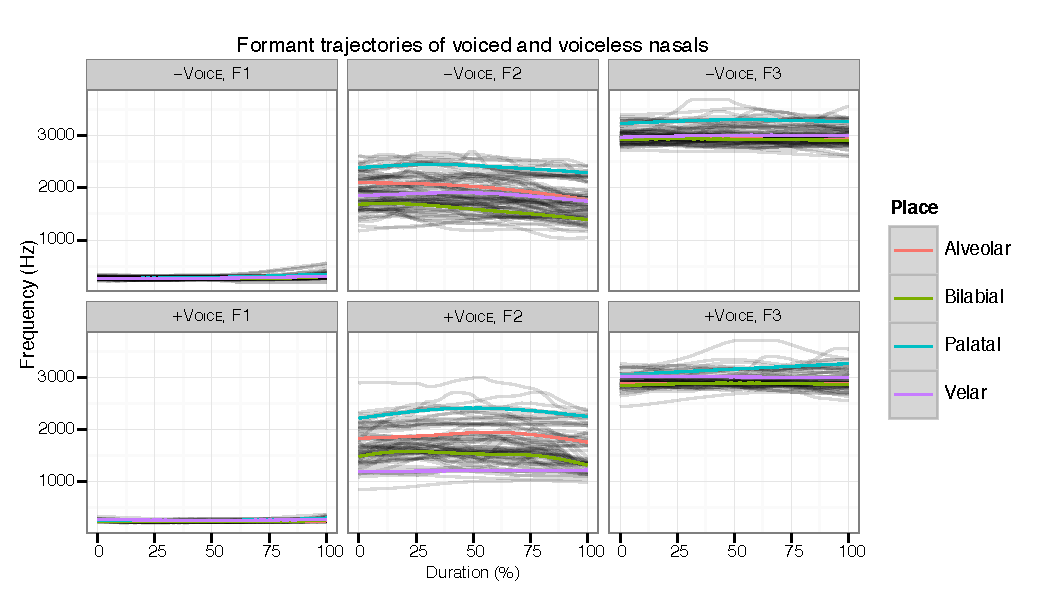
\includegraphics[scale=1.0]{figures/formants.pdf}
	\caption{First, second and third formant tracks of voiced nasals and voiced portions of voiceless nasals with normalised durations. Coloured lines represent locally weighted smoothed averages grouped by place of articulation.}
	\label{fig:formants}
\end{figure}

\newpage

For each token, mean formant values were computed over the middle 50\% of the voiced portions of a nasal segment and ANOVAs were performed with each of the formants.

\emph{F1}. Main effects were found for voice [$F(1, 125) = 76.3, p < .000$], place [$F(3, 125) = 8.03, p < .000$], condition [$F(2, 125) = 20.1, p < .000$] and tone [$F(3, 125) = 4.12, p = .008$]. Post-hoc analyses indicated significant differences in mean F1 values between voiced (\emph{M = } 245 Hz, \emph{SD} = 16 Hz) and voiceless (\emph{M = } 268 Hz, \emph{SD} = 21 Hz). Significant differences in mean F1 were found between palatal (\emph{M = } 268 Hz, \emph{SD} = 22 Hz) and bilabial (\emph{M = } 249 Hz, \emph{SD} = 18 Hz) nasals, and between palatal and alveolar nasals (\emph{M = } 256 Hz, \emph{SD} = 23 Hz). No other pairwise comparisons for place showed significant differences in F1; velar (\emph{M = } 268 Hz, \emph{SD} = 21 Hz). The mean F1 values by condition were all significantly different from each other: \condc (\emph{M = } 270 Hz, \emph{SD} = 22 Hz), \condf (\emph{M = } 258 Hz, \emph{SD} = 25 Hz), \condu (\emph{M = } 246 Hz, \emph{SD} = 12 Hz). Post-hoc analyses for tone indicated checked (\emph{M = } 263 Hz, \emph{SD} = 24 Hz) and high tones (\emph{M = } 253 Hz, \emph{SD} = 19 Hz) differed significantly from each other, but no other pairwise comparisons did; creaky (\emph{M = } 260 Hz, \emph{SD} = 25 Hz), low (\emph{M = } 252 Hz, \emph{SD} = 18 Hz).

\newpage

\emph{F2}. Main effects were found for voice [$F(1, 125) = 27.7, p < .000$], place [$F(3, 125) = 121.9, p < .000$] and condition [$F(2, 125) = 4.24, p = .012$], but not tone [$F(3, 125) = 1.73, p = .16$]. Tukey's HSD test for post hoc analyses indicated significant differences between voiced (\emph{M = } 1723 Hz, \emph{SD} = 358 Hz) and voiceless nasals (\emph{M = } 1884 Hz, \emph{SD} = 336 Hz). Other than the pairwise comparison between bilabial and velar nasals, all places of articulation were found to be significantly different from each other in their mean F2 values: alveolar (\emph{M = } 1942 Hz, \emph{SD} = 141 Hz), bilabial (\emph{M = } 1548 Hz, \emph{SD} = 153 Hz), palatal (\emph{M = } 2346 Hz, \emph{SD} = 163 Hz), velar (\emph{M = } 1668 Hz, \emph{SD} = 363 Hz). In elicitation condition comparisons, only \condc (\emph{M = } 1861 Hz, \emph{SD} = 381 Hz) and \condu (\emph{M = } 1733 Hz, \emph{SD} = 342 Hz) were found to differ significantly in mean F2 values; \condf (\emph{M = } 1839 Hz, \emph{SD} = 337 Hz).

\emph{F3.} Main effects were found for voice [$F(1, 125) = 8.61, p = .004$] and place [$F(3, 125) = 49.0, p < .000$], but not condition [$F(2, 125) = 0.99, p = .37$] and tone [$F(3, 125) = 2.84, p = .05$]. Post-hoc analyses indicated significant differences between voiced (\emph{M = } 2991 Hz, \emph{SD} = 151 Hz) and voiceless nasals (\emph{M = } 2943 Hz, \emph{SD} = 124 Hz). The mean F3 values of palatal nasals (\emph{M = } 3177 Hz, \emph{SD} = 103 Hz) were found to differ significantly from bilabial (\emph{M = } 2906 Hz, \emph{SD} = 79 Hz), alveolar (\emph{M = } 2916 Hz, \emph{SD} = 59 Hz) and velar nasals (\emph{M = } 2985 Hz, \emph{SD} = 173 Hz), of which the latter three did not differ significantly between each other.

\subsection{Pitch}

\emph{Data integrity.} Relative to formant tracking, the audio signal proved less problematic for the pitch tracker. After applying range [150, 300] and derivative maximum dF0$_{max}$ < 1 Hz/ms criteria, 204 of 247 tokens were retained for analyses. \Cref{fig:pitch} displays the resulting pitch tracks of voiced and voiceless nasals, normalised for duration.

\emph{Offset pitch.} To examine the effects of nasal segments on the onset pitch of the following vowel, the mean pitch for each token was calculated over the last 25\% of the segment. An ANOVA on mean offset pitch indicated main effects for voice [$F(1, 125) = 238, p < .000$], condition [$F(2, 125) = 19.7, p < .000$] and tone [$F(3, 125) = 3.46, p = .01$], but not place [$F(3, 125) = 0.36, p = .78$]. Post-hoc analyses showed that voiced (\emph{M = } 209 Hz, \emph{SD} = 5 Hz) and voiceless nasals (\emph{M = } 241 Hz, \emph{SD} = 26 Hz) differed significantly in their mean offset pitch. The \condu (\emph{M = } 211 Hz, \emph{SD} = 8 Hz) condition differed significantly from the other two, \condf (\emph{M = } 226 Hz, \emph{SD} = 28 Hz) and \condc (\emph{M = } 221 Hz, \emph{SD} = 21 Hz), which did not differ significantly from each other. For tone, creaky (\emph{M = } 224 Hz, \emph{SD} = 28 Hz) and low (\emph{M = } 217 Hz, \emph{SD} = 16 Hz) differed significantly from each other in mean offset pitch, though no other pairwise comparisons showed significant differences; checked (\emph{M = } 219 Hz, \emph{SD} = 20 Hz), high (\emph{M = } 219 Hz, \emph{SD} = 22 Hz).


\newpage
\begin{figure}[h!]
	% \vspace{2cm}
	\centering
	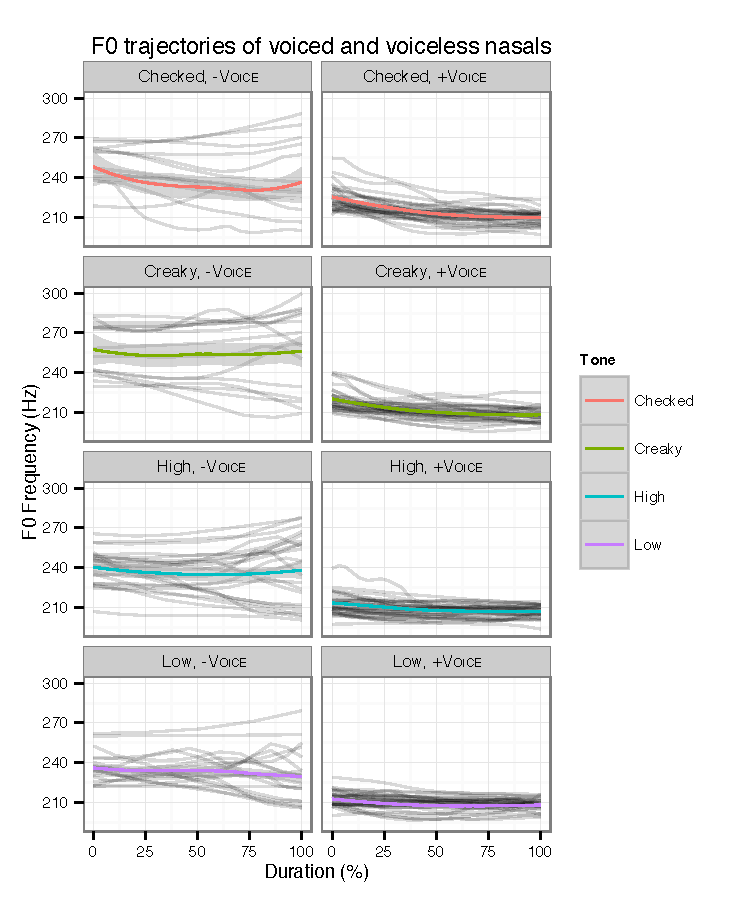
\includegraphics[scale=1.0]{figures/pitch.pdf}
	\caption{Pitch tracks of 204 tokens of voiced and voiceless nasals with normalised durations. Coloured lines represent locally weighted smoothed averages grouped by tone.}
	\label{fig:pitch}
\end{figure}

An additional analysis was carried out to verify that the above observed differences did not simply result from pitch variability in speech production between individual tokens. For each token, normalised pitch data were generated by subtracting the first F0 value from each of the following pitch data points in the token, that is setting the onset pitch to 0 Hz. An ANOVA on the mean offset normalised pitch replicated the above results, with main effects for voice [$F(1, 125) = 7.11, p = .008$], condition [$F(2, 125) = 4.43, p = .01$] and tone [$F(3, 125) = 5.76, p = .0009$], but not place [$F(3, 125) = 0.51, p = .69$].

\newpage

\subsection{EGG}

\emph{Data integrity.} As only time point data were extracted, peak detection on a smoothed EGG signal proved to be a relatively robust measure compared to pitch and formant tracking of acoustic data. All 247 tokens were analysed for their Contact Quotient (CQ) averages.

\emph{Mean CQ}. Mean contact quotients were calculated across the whole duration of voiced intervals of each token. An ANOVA indicated main effects for voice [$F(1, 125) = 34.0, p < .000$] and for condition [$F(2, 125) = 3.67, p = .03$], but not place [$F(3, 125) = 1.17, p = .32$] or tone [$F(3, 125) = 0.85, p = .47$]. Post-hoc analyses revealed that the mean CQ ratios were significantly higher in voiceless nasals (\emph{M = } 0.255, \emph{SD} = 0.0671) than in voiced nasals (\emph{M = } 0.219, \emph{SD} = 0.0211). The \condu (\emph{M = } 0.246, \emph{SD} = 0.0607) and \condc (\emph{M = } 0.228, \emph{SD} = 0.0375) differed significantly from each other though \condf (\emph{M = } 0.235, \emph{SD} = 0.0519) did not differ from either. \Cref{fig:egg} displays the uncollapsed means and standard deviations across the voice and condition variables.

\begin{figure}[h!]
	\centering
	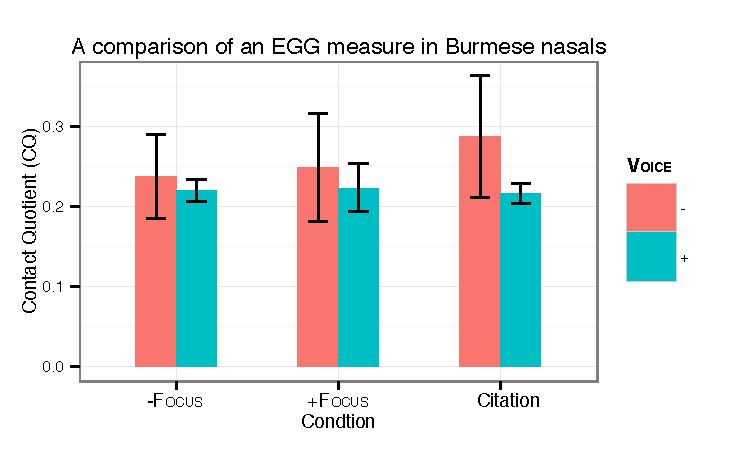
\includegraphics[scale=1.0]{figures/egg.pdf}
	\caption{Mean Contact Quotient (CQ) values for voiced and voiceless nasals across the three experimental conditions. Error bars represent one standard deviation.}
	\label{fig:egg}
\end{figure}

\newpage

\section{Discussion}

\emph{Data sparsity}. The relatively small power of the current dataset is particularly evident in viewing the results from the main effects and pairwise difference comparisons – that is, the dataset suggests a given variable (e.g. place) appears to have at least one difference between its levels (e.g. bilabial vs. alveolar), however, pairwise comparisons show few or inconsistent significant differences above the high levels of variance. Moreover, due to the number of data points, the ANOVAs conducted in the analyses did not model for neither second- (e.g. place and voice on mean F2) nor third-level (e.g. voice, condition and tone on mean F0 offset) interaction effects. However, several of the independent variables under investigation (e.g. voice and condition), showed consistently large effects across the different measures and thus general observations can still be made. Where specific differences lie within the different levels of the variables and the interaction behaviour between them, are questions that can only be addressed by future studies with additional participants. 

\emph{Formants.} Nasal formants pose considerable difficulty for automatic formant trackers and tokens elicited for the current project proved no exception to this. One way to recover additional data would be to do semi-supervised formant tracking with manual correction of tracks as necessary. A portion of the corrected data would then be checked for reliability by a second experimenter. This procedure, however, was something that was not feasible in the limited time and scope of this pilot study.

For F1, the current study found significant differences between the palatal and alveolar, and palatal and bilabial voiceless nasals but no others. While \citep{dantsuji1986some} did not elicit voiceless palatal nasals, he was not able to find consistent F1 differences across his three speakers. For F3, the current study found that, again, palatal nasals were significantly different from all three others. As \citep{dantsuji1986some} neither elicited palatal nasals nor reported statistical data on F3 values of the others, it is difficult to contextualise this finding. While the inconsistent F1 data may be explained by the lowered pitch during nasal segments, and the subsequent merging with F0 tracks, it is unclear why F3 resonances differ for palatals – but only with some other places, but not all.


For F2, however, the findings from the current data set are entirely consistent with previous results. \citet[][p. 5]{dantsuji1986some} found that bilabial and velar voiceless nasals differed significantly from alveolar voiceless nasals, though not each other. This was found for all three speakers. Similarly, the present study found that only bilabial and velar nasals do not differ in their mean F2 values while all other pairwise comparisons did (including the palatals). This finding suggests that place of articulation information is quite robustly encoded in the F2 frequencies.

\newpage
\emph{EGG Contact Quotient.}
In this study, it was found that there was a small but generally consistent difference in mean CQ values between voiced and voiceless nasals. Indeed, it has been found that a linguistic contrast through phonation need not necessarily be through large differences (e.g. breathy vs. modal voicing) and may still be perceptually salient to listeners. In a comparison of EGG measures on tense-lax phonation contrasts in three Loloish languages\footnote{Under some typlogical classifications, these languages and Burmese are classified under a Lolo-Burmese superfamily.} (Yi, Bo and Hani), \citet[][Appendix 2]{kuang2014vocal} reported similar CQ differences between the lax vs. tense conditions, respectively: Yi (\emph{M = } 0.40, \emph{SD} = 0.08 vs. \emph{M = } 0.46, \emph{SD} = 0.07), Bo (\emph{M = } 0.40, \emph{SD} = 0.06 vs. \emph{M = } 0.45, \emph{SD} = 0.06) and Hani (\emph{M = } 0.45, \emph{SD} = 0.06 vs. \emph{M = } 0.51, \emph{SD} = 0.06). That is, tense/lax phonations in these languages appear to be more like modal than creaky or breath phonations \citep[][p. 35]{kuang2014vocal}. \citet{kuang2014vocal} then applied the various metrics to a Yi stimuli set that was used in a perception study of various contrasts (vowel, tone, phonation) and found that CQ,\footnote{The first Principle Component (PC1) from a Principle Component Analysis of EGG pulse shape showed the strongest correlation ($r = 0.49, p < .001$). A PCA model was not fit to the current data due to time constraints.} correlated significantly with perceptual accuracy of the tense-lax phonationc contrast ($r = 0.35, p < .001$). Based on this result, the authors concluded that "the differences between tense and lax phonations are neither large nor extreme, but apparently consistent enough, and with robust enough acoustic consequences, to support this linguistic contrast." \citep[][p. 37]{kuang2014vocal}. With regard to the voiced/voiceless nasal contrast in Burmese, it may be the case that phonation differences serve as a perceptual cue, particularly in the absence of others (i.e. a period of voicelessness).

\emph{Offset pitch.} \citet{maddieson1984tono} reported overall pitch differences (25-44 Hz) at the onset of the following vowel between voiced and voiceless nasals across the different tones for tokens elicited in citation form. This result is replicated in the current study. In citation form, voiced and voiceless nasals showed overall differences in mean offset pitch (33-59 Hz) across the tones. An outstanding question from \citet{maddieson1984tono} pertained to whether the observed pitch differences arose from differences in laryngeal settings in the production of voiced and voiceless nasals. While differences in phonation were found between voiced and voiceless nasals, there appeared to be no significant correlation between mean pitch offset and mean CQ of the segment ($r = -0.09, p = .20$). While this result should be considered preliminary, it suggests that there are intrinsic pitch differences between voiced and voiceless nasals that are independent of at least one measure of laryngeal activity.

\newpage
\emph{Experimental conditions and duration results.} A number of studies have previously examined the durations of voiced and voiceless nasals in Burmese, though these studies elicited their tokens in only either citation \citep[\ipa{/\#NV\#/}][]{dantsuji1984study} or with a carrier phrase \citep[\condf in this study:][]{bhaskararao1991two}, but not both. This was the first study to do so and experimental condition was observed to be a consistently large effect across all the measures.

With the exception of F1, \condc and \condf never differed significantly from one other while \condc and \condu always did; significant differences between \condf and \condu varied from measure to measure. Two points are worthy of note from these results. Firstly, this is consistent with the nature of the utterances. In \condc the entire word is the phrase and all prominence is placed on the single stressed syllable. It is the opposite in the \condu condition. The elicited word receives the little prominence relative to other words in the sentence and the least compared to the two other conditions. Secondly, this suggests that the duration data and reported in the two previous studies as well as the present one are generally comparable, despite some differences in elicitation methods. Indeed, the three studies provide converging evidence that, firstly, Burmese voiceless nasals are longer than voiced nasals and that, secondly, voiced nasals are longer than the voiced portions of voiceless nasals.

\emph{Perception of voiceless nasals.} Though Burmese voiceless nasals have been suggested as 'textbook voiceless nasals' \citep[][p. 80]{bhaskararao1991two}, consisting of voiced and voiceless portions, the present data suggests this is not necessarily true. While \condc and \condf conditions elicited voiceless portions regularly (83\% and 73\%, respectively), none of the voiceless nasals in the \condu were produced with evident voicelessness. This finding, as well as the consistent effect of voice category on the various measures, brings into question the perceptual cues that signal the voice vs. voiceless nasal category distinction in Burmese, and the relative weighting of these cues. As per \citet{kuang2014vocal}, a possible companion study would be to use the elicited audio data as stimuli in an AXB discrimination task in order to compare correlations between perceptual accuracy and the various acoustic/EGG measures.

While it is true that more data must be gathered before the acoustic and EGG correlates of these segments can be accurately established, follow up studies may be able to gather perception and production data together in one session. Given the complexity of interacting variables, from voicing, tone, phonation to prosody, it will be important for future studies to distinguish between which of the acoustic/EGG correlates actually serve as linguistically relevant, i.e. phonological, cues from those which are not, i.e. phonetic.


\newpage
\section{Acknowledgements}

Many thanks go to Mike Proctor, Felicity Cox, Ivan Yuen and attendees of the Macquarie University Phonetics Lab for their feedback and help with all aspects of this project, from start to end. I would like to thank Ewald Enzinger for assistance with the formant and pitch trackers, and the very cooperative Burmese speaker who \lbrack was\rbrack \hspace{0.1em} volunteered for this study.

\onehalfspacing
\nocite{*}
\printbibliography

\singlespacing
\newpage
\section{Appendix A}

\begin{table}[h!]
\centering
\caption*{The list of stimulus words used elicitation in all three conditions.}
\label{tab:words}
	\begin{tabular}{cccccll}
	\toprule\\
	Burmese & IPA  & Place    & Voice  & Tone    & Gloss                     & POS      \\
	\midrule
	\burm{မ  }     & \ipa{ma̰}  & Bilabial & +     & Creaky  & to lift                   & verb     \\
	\burm{မာ  }    & \ipa{mà}  & Bilabial & +     & Low     & hard                      & adj      \\
	\burm{မား }    & \ipa{má}  & Bilabial & +     & High    & toweringly (intensifier)  & adv      \\
	\burm{မတ် }    & \ipa{maʔ}  & Bilabial & +     & Checked & upright, vertical         & adj      \\
	\burm{မှ  }    & \ipa{m̥a̰} & Bilabial & -     & Creaky  & locative                  & particle \\
	\burm{မှာ }    & \ipa{m̥à} & Bilabial & -     & Low     & order (buy)               & verb     \\
	\burm{မှား}    & \ipa{m̥á} & Bilabial & -     & High    & wrong                     & adj      \\
	\burm{မှတ်}    & \ipa{m̥aʔ} & Bilabial & -     & Checked & to mark                   & verb     \\
	\burm{န   }    & \ipa{na̰}  & Alveolar & +     & Creaky  & to be stupid              & verb     \\
	\burm{နာ  }    & \ipa{nà}  & Alveolar & +     & Low     & to suffer pain            & verb     \\
	\burm{နား }    & \ipa{ná}  & Alveolar & +     & High    & to rest                   & verb     \\
	\burm{နတ် }    & \ipa{naʔ}  & Alveolar & +     & Checked & lord                      & noun     \\
	\burm{နှ  }    & \ipa{n̥a̰} & Alveolar & -     & Creaky  & how many                  & particle \\
	\burm{နှာ }    & \ipa{n̥à} & Alveolar & -     & Low     & nose                      & noun     \\
	\burm{နှား}    & \ipa{n̥á} & Alveolar & -     & High    & \textsc{na}                        & \textsc{na}       \\
	\burm{နှတ်}    & \ipa{n̥aʔ} & Alveolar & -     & Checked & administer snuff          & verb     \\
	\burm{ည   }    & \ipa{ɲa̰}  & Palatal  & +     & Creaky  & night                     & noun     \\
	\burm{ညာ  }    & \ipa{ɲà}  & Palatal  & +     & Low     & right (side)              & noun     \\
	\burm{ညား }    & \ipa{ɲá}  & Palatal  & +     & High    & \textsc{na}                        & \textsc{na}       \\
	\burm{ညတ် }    & \ipa{ɲaʔ}  & Palatal  & +     & Checked & \textsc{na}                        & \textsc{na}       \\
	\burm{ညှ  }    & \ipa{ɲ̥a̰} & Palatal  & -     & Creaky  & \textsc{na}                        & \textsc{na}       \\
	\burm{ညှာ }    & \ipa{ɲ̥à} & Palatal  & -     & Low     & to be considerate         & verb     \\
	\burm{ညှား}    & \ipa{ɲ̥á} & Palatal  & -     & High    & \textsc{na}                        & \textsc{na}       \\
	\burm{ညှတ်}    & \ipa{ɲ̥aʔ} & Palatal  & -     & Checked & \textsc{na}                        & \textsc{na}       \\
	\burm{င   }    & \ipa{ŋa̰}  & Velar    & +     & Creaky  & be of sufficient quantity & verb     \\
	\burm{ငါ  }    & \ipa{ŋà}  & Velar    & +     & Low     & I (informal)              & pronoun  \\
	\burm{ငါး }    & \ipa{ŋá}  & Velar    & +     & High    & fish                      & noun     \\
	\burm{ငတ် }    & \ipa{ŋaʔ}  & Velar    & +     & Checked & to crave for              & verb     \\
	\burm{ငှ  }    & \ipa{ŋ̥a̰} & Velar    & -     & Creaky  & to distribute equally     & verb     \\
	\burm{ငှါ }    & \ipa{ŋ̥à} & Velar    & -     & Low     & possession/belonging      & noun     \\
	\burm{ငှါး}    & \ipa{ŋ̥á} & Velar    & -     & High    & to borrow                 & verb     \\
	\burm{ငှတ်}    & \ipa{ŋ̥aʔ} & Velar    & -     & Checked & \textsc{na}                        & \textsc{na}    \\
	\bottomrule  
	\end{tabular}
\end{table}

\end{document}